\documentclass[extendedabs]{bmvc2k}
\usepackage[]{graphicx}
\usepackage{times}
\usepackage{epsfig}
\usepackage{amsmath}
\usepackage{amssymb}
\usepackage{tabularx}
\usepackage{array}
\usepackage{rotating}
\usepackage{color}
\usepackage{enumerate}
\usepackage{booktabs}
\usepackage{url}
\captionsetup[subfigure]{labelformat=empty}  % remove (a),(b) etc subfloat labels

\title{Recognizing Image Style: Extended Abstract}
\def\httilde{\mbox{\tt\raisebox{-.5ex}{\symbol{126}}}}
\addauthor{Sergey Karayev}{}{1}
\addauthor{Matthew Trentacoste}{}{2}
\addauthor{Helen Han}{}{1}
\addauthor{Aseem Agarwala}{}{2}
\addauthor{Trevor Darrell}{}{1}
\addauthor{Aaron Hertzmann}{}{2}
\addauthor{Holger Winnemoeller}{}{2}
\addinstitution{University of California, Berkeley}
\addinstitution{Adobe}


\begin{document}
\maketitle

\noindent
Deliberately-created images convey meaning, and \textit{visual style} is often a significant component of image meaning.
For example, a political candidate portrait made in the lush colors of a Renoir painting tells a different story than if it were in the harsh, dark tones of a horror movie.
While understanding style is crucial to image understanding, very little research in computer vision has explored visual style.

We present two novel datasets of image style, describe an approach to predicting style of images, and perform a thorough evaluation of different image features for these tasks.
We find that features learned in a multi-layer network generally perform best -- even when trained with object class (not style) labels.
Our approach shows excellent classification performance on both datasets, and we use the learned classifiers to extend traditional tag-based image search to consider stylistic constraints.

%%%
\newcommand{\wid}{.7in}
\newcommand{\fgap}{.57in}
\newcommand{\dgap}{.42in}

\paragraph{Flickr Style}
Using curated Flickr Groups, we gather 80K photographs annotated with 20 style labels, ranging from photographic techniques  (``Macro,'' ``HDR''), composition styles (``Minimal,'' ``Geometric''), moods (``Serene,'' ``Melancholy''), genres (``Vintage,'' ``Romantic,'' ``Horror''), to types of scenes (``Hazy,'' ``Sunny'').

Top five predictions on the test set for a selection of styles:

\vspace{.666em}{\centering
\begin{tabular}{m{.02in}|m{\fgap} m{\fgap} m{\fgap} m{\fgap} m{\fgap}}
    \begin{turn}{90}\small{Minimal}\end{turn} &
    
\includegraphics[width=\wid]{../../figures/flickr_on_flickr/pred_style_Minimal/w/0.jpg} &
    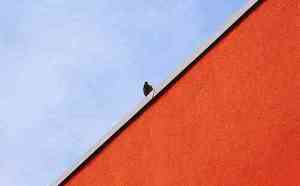
\includegraphics[width=\wid]{../../figures/flickr_on_flickr/pred_style_Minimal/w/1.jpg} &
    
\includegraphics[width=\wid]{../../figures/flickr_on_flickr/pred_style_Minimal/w/2.jpg} &
    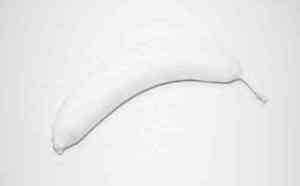
\includegraphics[width=\wid]{../../figures/flickr_on_flickr/pred_style_Minimal/w/3.jpg} \\
    \begin{turn}{90}\tiny{Depth of Field}\end{turn} &
    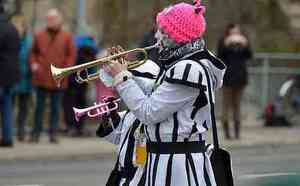
\includegraphics[width=\wid]{../../figures/flickr_on_flickr/pred_style_Depth_of_Field/w/0.jpg} &
    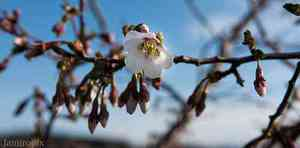
\includegraphics[width=\wid]{../../figures/flickr_on_flickr/pred_style_Depth_of_Field/w/1.jpg} &
    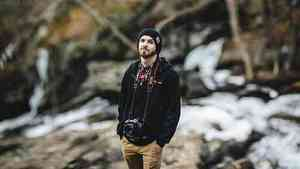
\includegraphics[width=\wid]{../../figures/flickr_on_flickr/pred_style_Depth_of_Field/w/2.jpg} &
    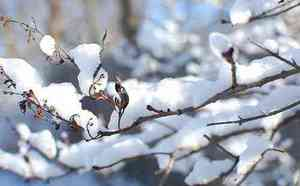
\includegraphics[width=\wid]{../../figures/flickr_on_flickr/pred_style_Depth_of_Field/w/3.jpg} \\
    \begin{turn}{90}\footnotesize{Melancholy}\end{turn} &
    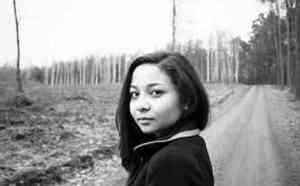
\includegraphics[width=\wid]{../../figures/flickr_on_flickr/pred_style_Melancholy/w/0.jpg} &
    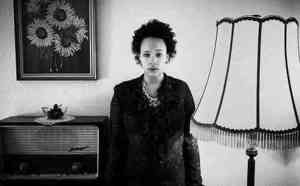
\includegraphics[width=\wid]{../../figures/flickr_on_flickr/pred_style_Melancholy/w/2.jpg} &
    
\includegraphics[width=\wid]{../../figures/flickr_on_flickr/pred_style_Melancholy/w/3.jpg} &
    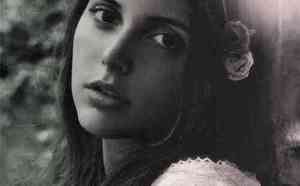
\includegraphics[width=\wid]{../../figures/flickr_on_flickr/pred_style_Melancholy/w/4.jpg} \\
    \begin{turn}{90}\footnotesize{HDR}\end{turn} &
    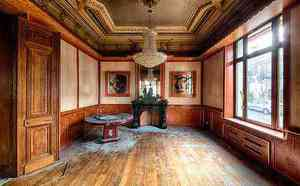
\includegraphics[width=\wid]{../../figures/flickr_on_flickr/pred_style_HDR/w/0.jpg} &
    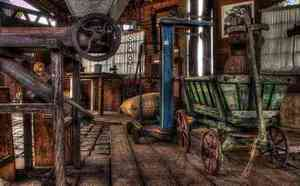
\includegraphics[width=\wid]{../../figures/flickr_on_flickr/pred_style_HDR/w/2.jpg} &
    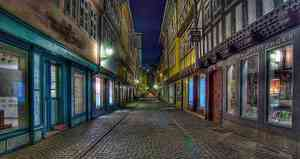
\includegraphics[width=\wid]{../../figures/flickr_on_flickr/pred_style_HDR/w/3.jpg} &
    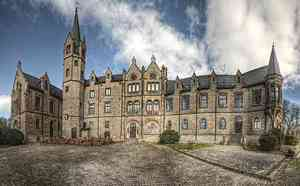
\includegraphics[width=\wid]{../../figures/flickr_on_flickr/pred_style_HDR/w/4.jpg} \\
    \begin{turn}{90}\small{Vintage}\end{turn} &
    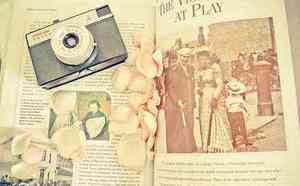
\includegraphics[width=\wid]{../../figures/flickr_on_flickr/pred_style_Vintage/w/0.jpg} &
    
\includegraphics[width=\wid]{../../figures/flickr_on_flickr/pred_style_Vintage/w/2.jpg} &
    
\includegraphics[width=\wid]{../../figures/flickr_on_flickr/pred_style_Vintage/w/3.jpg} &
    
\includegraphics[width=\wid]{../../figures/flickr_on_flickr/pred_style_Vintage/w/4.jpg} \\
\end{tabular}
}


%%%
\paragraph{Wikipaintings}
Using community-annotated data, we gather 85K\\
paintings annotated with 25 style/genre labels.

Top five predictions on the test set for a selection of styles:

\vspace{.666em}{\centering
\begin{tabular}{m{.02in}|m{\fgap} m{\fgap} m{\fgap} m{\fgap} m{\fgap}}
    \begin{turn}{90}\small{Baroque}\end{turn} &
    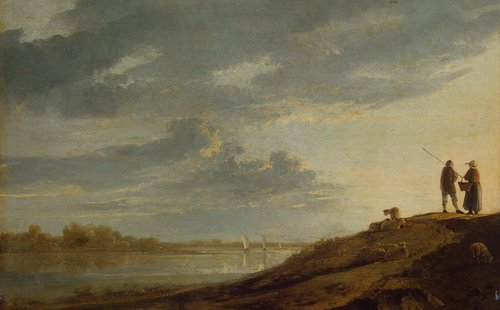
\includegraphics[width=\wid]{../../figures/wp_on_wp/style_Baroque/w/0.jpg} &
    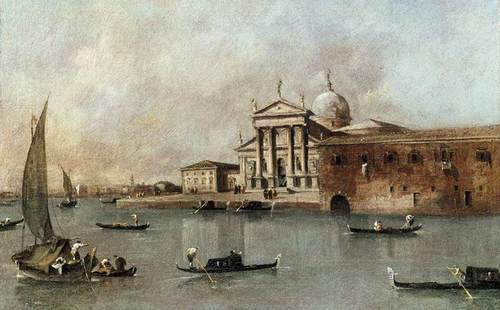
\includegraphics[width=\wid]{../../figures/wp_on_wp/style_Baroque/w/1.jpg} &
    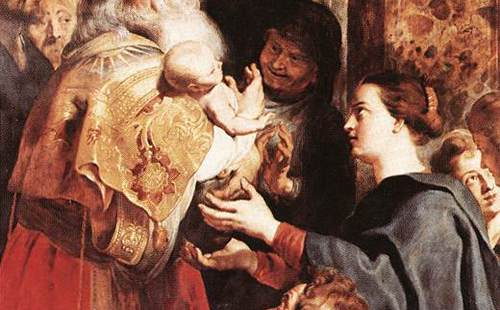
\includegraphics[width=\wid]{../../figures/wp_on_wp/style_Baroque/w/2.jpg} &
    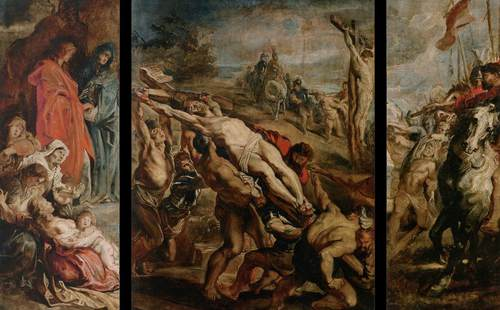
\includegraphics[width=\wid]{../../figures/wp_on_wp/style_Baroque/w/4.jpg} \\
    \begin{turn}{90}\tiny{Impressionism}\end{turn} &
    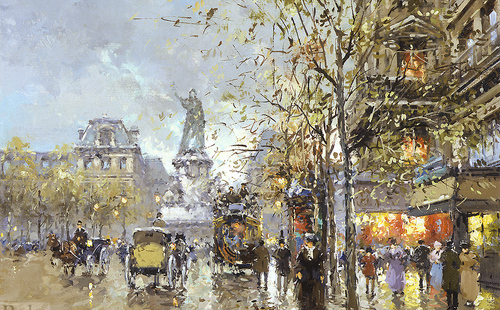
\includegraphics[width=\wid]{../../figures/wp_on_wp/style_Impressionism/w/0.jpg} &
    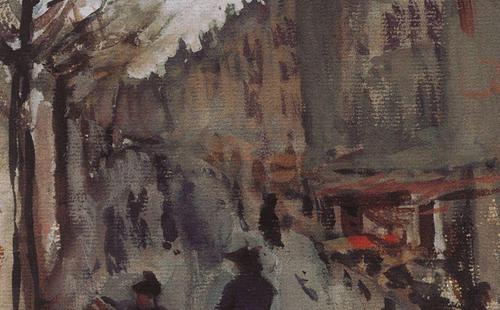
\includegraphics[width=\wid]{../../figures/wp_on_wp/style_Impressionism/w/1.jpg} &
    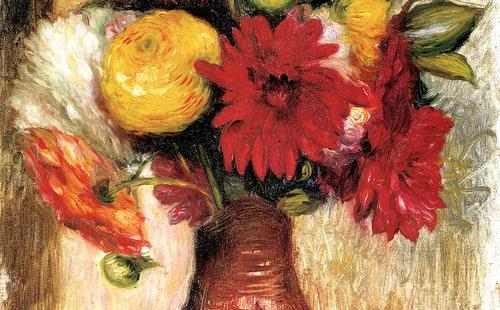
\includegraphics[width=\wid]{../../figures/wp_on_wp/style_Impressionism/w/2.jpg} &
    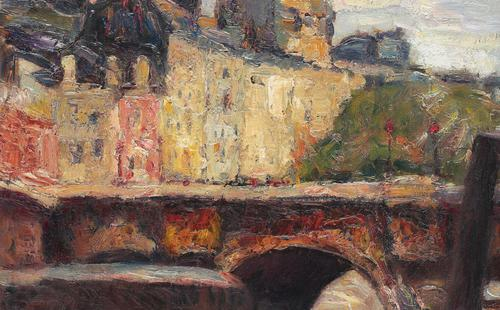
\includegraphics[width=\wid]{../../figures/wp_on_wp/style_Impressionism/w/3.jpg} \\
    \begin{turn}{90}\footnotesize{Ukiyo-e}\end{turn} &
    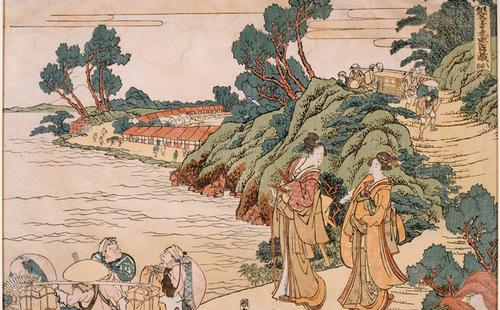
\includegraphics[width=\wid]{../../figures/wp_on_wp/style_Ukiyo-e/w/0.jpg} &
    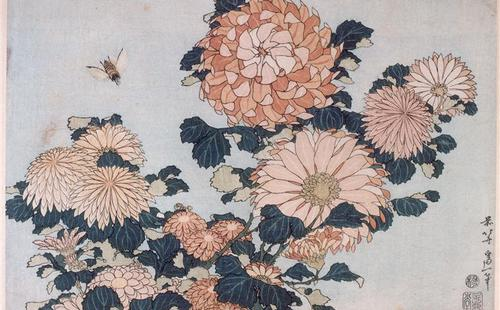
\includegraphics[width=\wid]{../../figures/wp_on_wp/style_Ukiyo-e/w/1.jpg} &
    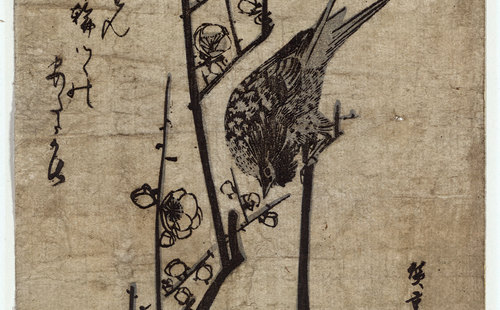
\includegraphics[width=\wid]{../../figures/wp_on_wp/style_Ukiyo-e/w/2.jpg} &
    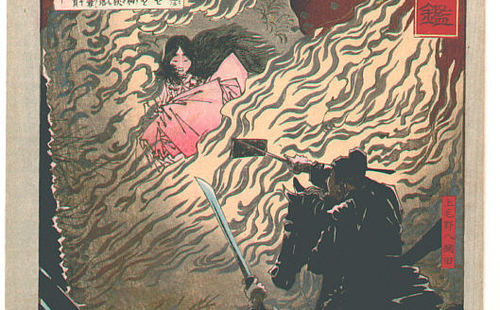
\includegraphics[width=\wid]{../../figures/wp_on_wp/style_Ukiyo-e/w/3.jpg} \\
    \begin{turn}{90}\small{Cubism}\end{turn} &
    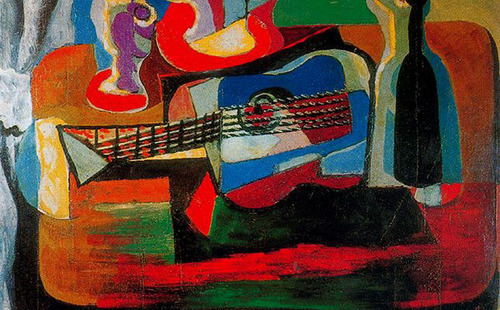
\includegraphics[width=\wid]{../../figures/wp_on_wp/style_Cubism/w/0.jpg} &
    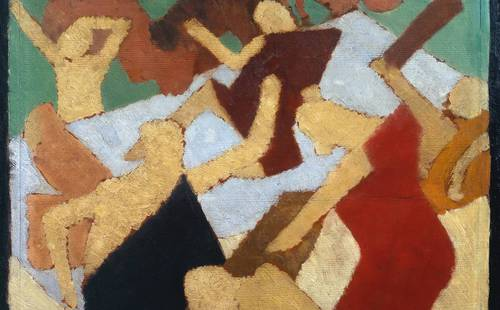
\includegraphics[width=\wid]{../../figures/wp_on_wp/style_Cubism/w/1.jpg} &
    
\includegraphics[width=\wid]{../../figures/wp_on_wp/style_Cubism/w/2.jpg} &
    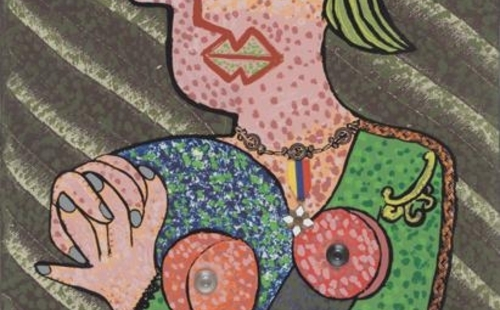
\includegraphics[width=\wid]{../../figures/wp_on_wp/style_Cubism/w/3.jpg} \\
    \begin{turn}{90}\footnotesize{Color Field}\end{turn} &
    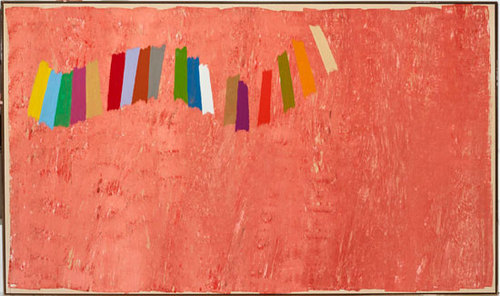
\includegraphics[width=\wid]{../../figures/wp_on_wp/style_Color_Field_Painting/w/0.jpg} &
    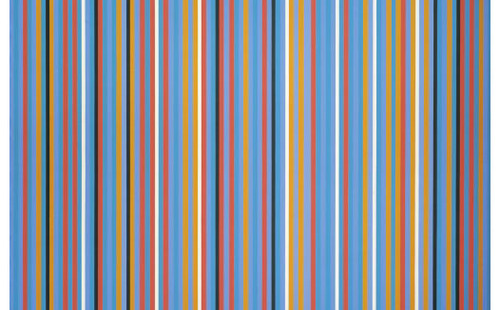
\includegraphics[width=\wid]{../../figures/wp_on_wp/style_Color_Field_Painting/w/1.jpg} &
    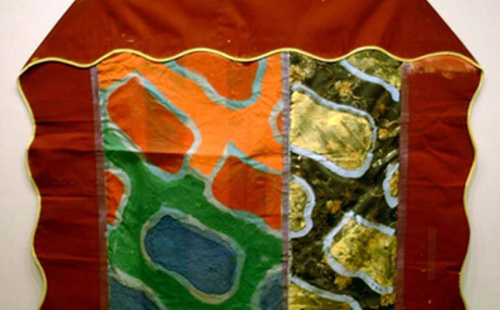
\includegraphics[width=\wid]{../../figures/wp_on_wp/style_Color_Field_Painting/w/2.jpg} &
    
\includegraphics[width=\wid]{../../figures/wp_on_wp/style_Color_Field_Painting/w/4.jpg} \\
\end{tabular}
}


\newpage

%%%
\paragraph{Features and Learning}
We test the following features: \textbf{L*a*b color} histogram, \textbf{GIST} descriptor, Graph-based \textbf{visual saliency}, Meta-class binary (\textbf{MC-bit}) object features, and deep convolutional neural networks (CNN), using the Caffe implementation of Krizhevsky's ImageNet architeture (referred to as the \textbf{DeCAF} feature, with subscript denoting network layer).
Notably, the last two of these are features designed and trained for object recognition.

As we hypothesize that style features may be content dependent, we also train \textbf{Content} classifiers using the CNN features and an aggregated version of the PASCAL VOC dataset, and use them in second-stage fusion with other features.

%%%
\paragraph{Evaluation}
Mean APs on three datasets for the considered single-channel features and their second-stage combination.
Only the clearly superior features are evaluated on the Flickr and Wikipaintings datasets.

{\footnotesize {\centering
\vspace{1em}
\begin{tabular}{lrrrrrrrrr}
\toprule
{}                & \begin{tabular}[x]{@{}c@{}}Fusion x\\Content\end{tabular} & DeCAF$_6$ & MC-bit & L*a*b* Hist & GIST  & random \\
\midrule
AVA Style         & \textbf{0.581}   & 0.579     & 0.539  & 0.288       & 0.220 & 0.132 \\
Flickr            & \textbf{0.368}   & 0.336     & 0.328  & -           & -     & 0.052 \\
Wikipaintings     & \textbf{0.473}   & 0.356     & 0.441  & -           & -     & 0.043 \\
\bottomrule
\end{tabular}
}
}

\vspace{.666em}
We compare our predictors to human observers, using Amazon Mechanical Turk experiments, and find that our classifiers predict Group membership at essentially the same level of accuracy as Turkers.
We also test on the AVA aesthetic prediction task, and show that using the ``deep'' object recognition features improves over state-of-the-art results.

\paragraph{Applications}
Example of filtering image search results by style.
Our Flickr Style classifiers are applied to images found on Pinterest.
The images are searched by the text contents of their captions, then filtered by the response of the style classifiers.
Here we show top five results for the query ``Dress.''

{\centering
    \begin{tabular}{m{.02in}|m{\dgap} m{\dgap} m{\dgap} m{\dgap} m{\dgap}}
    \begin{turn}{90}{Pastel}\end{turn} &
    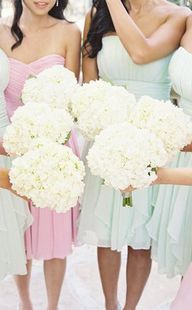
\includegraphics[width=.53in]{../../figures/flickr_on_pinterest/dress/pred_style_Pastel/h/0.jpg} &
    
\includegraphics[width=.53in]{../../figures/flickr_on_pinterest/dress/pred_style_Pastel/h/1.jpg} &
    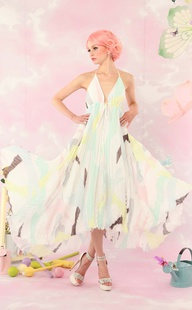
\includegraphics[width=.53in]{../../figures/flickr_on_pinterest/dress/pred_style_Pastel/h/2.jpg} &
    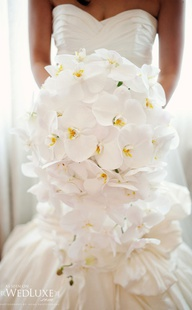
\includegraphics[width=.53in]{../../figures/flickr_on_pinterest/dress/pred_style_Pastel/h/3.jpg} &
    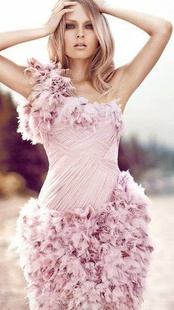
\includegraphics[width=.53in]{../../figures/flickr_on_pinterest/dress/pred_style_Pastel/h/4.jpg} \\ \\
    \begin{turn}{90}{Ethereal}\end{turn} &
    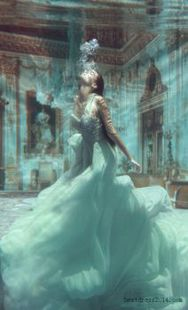
\includegraphics[width=.53in]{../../figures/flickr_on_pinterest/dress/pred_style_Ethereal/h/0.jpg} &
    
\includegraphics[width=.53in]{../../figures/flickr_on_pinterest/dress/pred_style_Ethereal/h/1.jpg} &
    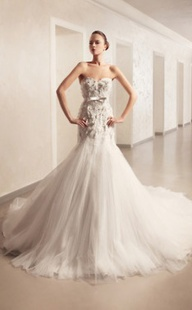
\includegraphics[width=.53in]{../../figures/flickr_on_pinterest/dress/pred_style_Ethereal/h/2.jpg} &
    
\includegraphics[width=.53in]{../../figures/flickr_on_pinterest/dress/pred_style_Ethereal/h/3.jpg} &
    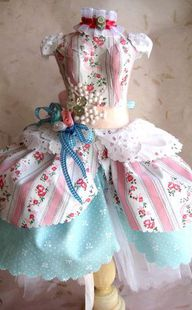
\includegraphics[width=.53in]{../../figures/flickr_on_pinterest/dress/pred_style_Ethereal/h/4.jpg} \\ \\
    \begin{turn}{90}{Noir}\end{turn} &
    \includegraphics[width=.53in]{../../figures/flickr_on_pinterest/dress/pred_style_Noir/h/0.jpg} &
    \includegraphics[width=.53in]{../../figures/flickr_on_pinterest/dress/pred_style_Noir/h/1.jpg} &
    \includegraphics[width=.53in]{../../figures/flickr_on_pinterest/dress/pred_style_Noir/h/2.jpg} &
    \includegraphics[width=.53in]{../../figures/flickr_on_pinterest/dress/pred_style_Noir/h/3.jpg} &
    \includegraphics[width=.53in]{../../figures/flickr_on_pinterest/dress/pred_style_Noir/h/4.jpg} \\ \\
    \end{tabular}
}


\paragraph{Code \& Data}
All data, trained predictors, and code are available at\\
{\small \url{http://sergeykarayev.com/recognizing-image-style/}}.

\end{document}
